\documentclass[conference]{IEEEtran}

\usepackage[T1]{fontenc}
\usepackage[utf8]{inputenc}
\usepackage{graphicx}
\usepackage{adjustbox}
\usepackage{amsmath}
\usepackage{array}
\usepackage{url}
\usepackage{cite}
\usepackage{balance}

\graphicspath{{../report_assets/figures/}}
\hyphenation{re-pro-duc-i-bil-i-ty class-i-fi-ca-tion}

\begin{document}

\title{Text Classification Pipeline Forensics:\\
Reproducibility, Shortcut Sensitivity, and Data Quality in Disaster Tweets}

\author{\IEEEauthorblockN{LAI Jiaxing}
\and
\IEEEauthorblockN{HE Jiarui}}

\maketitle

\begin{abstract}
This project investigates when apparent improvements to a disaster-tweet classifier are reproducible and trustworthy rather than products of split drift, superficial shortcuts, operating-point changes, or label inconsistency. All experiments used 7,613 labeled tweets and one immutable, stable-ID partition of 4,567 training, 1,523 development (dev), and 1,523 held-out examples. Ticket decisions were made from train/dev evidence, frozen, and only then reported on held-out data. A raw-text word-unigram TF--IDF plus Logistic Regression baseline achieved held-out target-class F1 of 0.749186, missing the supplied reference 0.757422 by 0.008236, although the local pipeline was deterministic and leakage-controlled. URL placeholdering produced a small, precision-oriented improvement and exact invariance under a paired URL perturbation. A higher-scoring shallow-feature model was rejected because masking keyword metadata changed 702 dev predictions and reduced F1 from 0.749396 to 0.642306. Balanced Logistic Regression was selected on dev as a recall-oriented operating point; on held-out it achieved precision 0.744361, recall 0.756881, F1 0.750569, and accuracy 0.783979, while fixing 35 baseline false negatives and introducing 56 false positives. A subsequent duplicate and label audit found substantial cross-split relationships and conflicting annotations, but an eight-row in-memory correction probe reduced dev F1 and was rejected. The final frozen model therefore retains the balanced classifier with no label corrections. Five clean-process replays reproduced labels and metrics with maximum score drift $1.11\times10^{-16}$. The results show that score changes require transition, robustness, provenance, and case evidence; they do not establish universal deployment superiority.
\end{abstract}

\begin{IEEEkeywords}
text classification, reproducibility, error analysis, dataset shortcuts, decision thresholds, data quality
\end{IEEEkeywords}

\section{Project Problem and Goal}

\subsection{Problem Context and Forensic Goal}

The task is binary classification of the Kaggle Disaster Tweets data: target 1 denotes a tweet labeled as describing a real disaster and target 0 denotes a tweet labeled otherwise \cite{kaggle-dataset,ucbrise-mirror,project-handout}. The assignment is deliberately forensic. A higher aggregate score can arise because a transformation removed nuisance variation, because a decision threshold happened to fit the metric, because metadata exposed a benchmark shortcut, or because inconsistent labels changed what the metric rewards. Score differences alone therefore cannot determine whether a pipeline change is trustworthy.

The project goal was to connect each proposed change to four kinds of evidence: a controlled intended lever, dev-set metric and transition behavior, row-level examples with stable IDs, and a frozen post-selection held-out report. Five tickets covered baseline reproduction, text normalization, shallow-feature shortcuts, decision rules and classifier choices, and data quality. The unifying question was not simply which row of a score table was largest, but which conclusions remained defensible when the prediction movements, perturbation behavior, data provenance, and unresolved uncertainty were considered together.

This report distinguishes observation from interpretation. Metrics, counts, scores, IDs, and hashes are observations regenerated from repository artifacts. Conclusions such as ``shortcut-sensitive,'' ``recall-oriented,'' or ``potential annotation issue'' are bounded interpretations of those observations. They are not causal claims and do not replace external label adjudication.

\subsection{Evidence Contributions}

The project contributes: (1) a deterministic majority floor and raw-text TF--IDF baseline audit; (2) six isolated normalization comparisons plus a raw control; (3) ten text, metadata, and shallow-feature comparisons with targeted perturbations; (4) a bounded threshold, regularization, class-weight, and LinearSVC study; (5) exact, canonical, and bounded near-duplicate analyses with a controlled label-correction probe; and (6) a frozen-decision replay audit. All prediction transitions use Ticket 1 as the common comparator, as required by the instructor clarification \cite{instructor-clarifications}. These are project-specific contributions on one fixed benchmark, not claims of a novel classifier or broad external generalization.

\section{Methodology}

\subsection{Dataset and Fixed Split}

The labeled CSV contains the fields \texttt{id}, \texttt{keyword}, \texttt{location}, \texttt{text}, and \texttt{target}. The 7,613 IDs are unique. The instructor-provided split assigns each stable ID exactly once to train, dev, or held-out, with no ID overlap. Table~\ref{tab:dataset_split} gives the class counts. Train is the only fitting partition. Dev is the only partition used to choose preprocessing, features, hyperparameters, class weights, or thresholds. Held-out is restricted to reporting after a ticket decision is frozen \cite{starter-readme,starter-data}.

\begin{table*}[t]
\centering
\caption{Dataset and Fixed Split Statistics}
\label{tab:dataset_split}
\begin{adjustbox}{max width=\textwidth}
\scriptsize
\begin{tabular}{lrrrrrr}
\hline
split & rows & target 0 & target 1 & target 1 rate & unique ids & seed \\
\hline
train & 4567 & 2605 & 1962 & 0.429604 & 4567 & 3102 \\
dev & 1523 & 868 & 655 & 0.430072 & 1523 & 3102 \\
heldout & 1523 & 869 & 654 & 0.429416 & 1523 & 3102 \\
\hline
\end{tabular}
\end{adjustbox}
\par\footnotesize{Counts are tweets; target-1 rate is a fraction in [0,1]. The split is fixed and stratified.}
\end{table*}


The split is stratified with seed 3102. ID-based joins were used throughout; dataframe position was never treated as identity. This prevents row-order changes from silently changing a comparison. The source-data SHA-256 is \texttt{61111c6d...60df}, and the split SHA-256 is \texttt{db2fd1fd...88f1}; full values remain in the frozen manifest. ID disjointness does not imply semantic independence, however: Ticket 5 found exact and approximate text relationships across splits.

\subsection{Metrics and Common Comparator}

Target 1 is the positive class. For true positives $TP$, false positives $FP$, false negatives $FN$, and true negatives $TN$, the reported measures are
\begin{align}
P &= \frac{TP}{TP+FP}, &
R &= \frac{TP}{TP+FN},\\
F_1 &= \frac{2PR}{P+R}, &
A &= \frac{TP+TN}{TP+TN+FP+FN}.
\end{align}
All metric values are unitless. Confusion and transition entries are tweet counts. The default probability rule is inclusive at threshold 0.50. A \emph{fixed FP} is a target-0 row predicted 1 by Ticket 1 and 0 by a candidate; a \emph{new FP} moves in the opposite direction. Fixed and new FNs are defined analogously for target-1 rows. These categories describe different semantic costs and are never netted into a single ``errors changed'' value.

F1 is the primary declared selection metric, but it contains no deployment-specific cost model. Accuracy and the full confusion matrix are retained so that recall gains cannot be presented without their precision and false-positive costs. Stable-ID change tables supply the complementary case evidence.

\subsection{Selection, Freeze, and Held-Out Policy}

Each ticket followed the same chronology: predeclare the question and bounded candidates; fit only on train; evaluate and interpret on dev; write an immutable decision artifact; then perform or reuse a post-freeze held-out report. Every frozen record states that held-out was not used for selection and that reopening was not permitted. Tickets 3 and 5 intentionally reuse previously validated prediction cores because their dev decisions retained an earlier model. This avoids unnecessary refitting while preserving ticket provenance.

Two later actions are explicitly separated from model selection. First, after a documented rollback removed Ticket 1 row-level artifacts, one authorized recovery replay reconstructed them with the exact frozen recipe. The historical primary comparison count remained one, and no parameter was changed. Second, after all five decisions were frozen, five distinct clean processes replayed the final recipes for audit only. Neither action reopened a decision. Procedural provenance is important because artifacts from earlier tickets existed during later work; the protection is a documented freeze policy, not a claim that every prior score was literally unknown.

\subsection{Floor, Baseline, and Reproducibility Controls}

The floor predicts the train-majority class, target 0, for every row. On dev it therefore has target-1 precision, recall, and F1 of zero, accuracy 0.569928, and confusion counts $868/0/655/0$ for $TN/FP/FN/TP$. Its role is wiring validation rather than competition.

The stronger baseline uses raw tweet text only, default lowercase word-unigram TF--IDF, and Logistic Regression with $C=1$, no class weighting, the \texttt{lbfgs} solver, \texttt{max\_iter}=100, threshold 0.50, and random state 3102. No metadata, manual normalization, threshold tuning, or train-plus-dev vocabulary fitting is used. Two independent baseline dev fits produced identical IDs, labels, scores, metrics, warnings, and iteration counts; the selected fit converged in 15 iterations. Table~\ref{tab:baseline_reference} separates the dev floor and baseline from the later reference comparison.

\begin{table*}[t]
\centering
\caption{Baseline Floor and Assignment-Reference Comparison}
\label{tab:baseline_reference}
\begin{adjustbox}{max width=\textwidth}
\scriptsize
\begin{tabular}{lrrrrrr}
\hline
condition & split & metric & value & reference or tolerance & absolute gap & within tolerance \\
\hline
train\_majority\_floor & dev & f1\_target\_1 & 0 & -- & -- & -- \\
raw\_text\_tfidf\_logistic\_regression & dev & f1\_target\_1 & 0.738812 & -- & -- & -- \\
frozen\_baseline\_heldout & heldout & heldout\_f1\_target\_1 & 0.749186 & 0.757422 & 0.008236 & False \\
\hline
\end{tabular}
\end{adjustbox}
\par\footnotesize{F1 is unitless in [0,1]. The assignment reference tolerance is 0.001; the frozen held-out result does not match it.}
\end{table*}


The locked audit environment recorded CPython 3.13.0, scikit-learn 1.9.0, pandas 3.0.3, NumPy 2.5.1, Matplotlib 3.11.1, and one CPU thread where supported \cite{sklearn-software,pandas-software,numpy-software,matplotlib-software}. Locked local reproducibility does not imply byte-identical probabilities on arbitrary systems or future package versions.

\subsection{Controlled Ticket Design}

Tickets 2--5 changed one intended lever or one explicitly declared bundle while retaining the fixed split and comparator. Ticket 2 enabled one surface transformation at a time. Ticket 3 isolated metadata families and declared text-feature combinations. Ticket 4 retained the raw text representation while changing one threshold, regularization, class-weight, or classifier lever. Ticket 5 changed only eight proposed training labels in an in-memory candidate; duplicate discovery and audit dispositions were not hidden training interventions. Candidate grids were bounded and evaluated on one fixed dev split, so they support controlled comparisons rather than exhaustive optimization.

\section{Main Evidence and Results}

\subsection{Cross-Ticket Quantitative Overview}

Table~\ref{tab:five_ticket_summary} summarizes the five frozen decisions. Tables~\ref{tab:dev_metrics} and \ref{tab:heldout_metrics} give the full selected dev and held-out metrics; Table~\ref{tab:confusion_summary} makes the error-count tradeoffs explicit. Table~\ref{tab:prediction_transitions} reports every ticket relative to the same Ticket 1 comparator. Ticket 1 equals Ticket 3 by deliberate retention, and Tickets 4 and 5 share a prediction core because Ticket 5 rejected corrections. These repeated rows are provenance facts rather than independent experimental replications.

\begin{table*}[t]
\centering
\caption{Project-Wide Results Across Five Tickets}
\label{tab:five_ticket_summary}
\begin{adjustbox}{max width=\textwidth}
\scriptsize
\begin{tabular}{lrrrrrrrr}
\hline
ticket & model name & dev f1 & heldout f1 & heldout accuracy & fixed fp & fixed fn & new fp & new fn \\
\hline
1 & raw\_text\_tfidf\_logistic\_regression & 0.738812 & 0.749186 & 0.797768 & 0 & 0 & 0 & 0 \\
2 & normalize\_urls\_placeholder & 0.740313 & 0.753117 & 0.804990 & 22 & 8 & 4 & 15 \\
3 & raw\_text\_tfidf\_logistic\_regression & 0.738812 & 0.749186 & 0.797768 & 0 & 0 & 0 & 0 \\
4 & lr\_c1\_balanced\_default & 0.752085 & 0.750569 & 0.783979 & 0 & 35 & 56 & 0 \\
5 & lr\_c1\_balanced\_default & 0.752085 & 0.750569 & 0.783979 & 0 & 35 & 56 & 0 \\
\hline
\end{tabular}
\end{adjustbox}
\par\footnotesize{Metrics are recomputed from archived predictions. Transition counts are held-out changes relative to Ticket 1; counts are tweets.}
\end{table*}

\begin{table*}[t]
\centering
\caption{Selected Dev Metrics by Ticket}
\label{tab:dev_metrics}
\begin{adjustbox}{max width=\textwidth}
\scriptsize
\begin{tabular}{lrrrrrrrr}
\hline
ticket & precision target 1 & recall target 1 & f1 target 1 & accuracy & true negative & false positive & false negative & true positive \\
\hline
1 & 0.790941 & 0.693130 & 0.738812 & 0.789232 & 748 & 120 & 201 & 454 \\
2 & 0.804659 & 0.685496 & 0.740313 & 0.793171 & 759 & 109 & 206 & 449 \\
3 & 0.790941 & 0.693130 & 0.738812 & 0.789232 & 748 & 120 & 201 & 454 \\
4 & 0.746988 & 0.757252 & 0.752085 & 0.785292 & 700 & 168 & 159 & 496 \\
5 & 0.746988 & 0.757252 & 0.752085 & 0.785292 & 700 & 168 & 159 & 496 \\
\hline
\end{tabular}
\end{adjustbox}
\par\footnotesize{Precision, recall, F1, and accuracy are unitless in [0,1]; confusion entries are tweet counts. Selection used dev evidence.}
\end{table*}

\begin{table*}[t]
\centering
\caption{Frozen Held-Out Metrics by Ticket}
\label{tab:heldout_metrics}
\begin{adjustbox}{max width=\textwidth}
\scriptsize
\begin{tabular}{lrrrrrrrr}
\hline
ticket & precision target 1 & recall target 1 & f1 target 1 & accuracy & true negative & false positive & false negative & true positive \\
\hline
1 & 0.801394 & 0.703364 & 0.749186 & 0.797768 & 755 & 114 & 194 & 460 \\
2 & 0.825137 & 0.692661 & 0.753117 & 0.804990 & 773 & 96 & 201 & 453 \\
3 & 0.801394 & 0.703364 & 0.749186 & 0.797768 & 755 & 114 & 194 & 460 \\
4 & 0.744361 & 0.756881 & 0.750569 & 0.783979 & 699 & 170 & 159 & 495 \\
5 & 0.744361 & 0.756881 & 0.750569 & 0.783979 & 699 & 170 & 159 & 495 \\
\hline
\end{tabular}
\end{adjustbox}
\par\footnotesize{Metrics are descriptive held-out results after dev-only freezing; they were not used to reopen selection.}
\end{table*}

\begin{table*}[t]
\centering
\caption{Selected Dev and Held-Out Confusion-Matrix Counts}
\label{tab:confusion_summary}
\begin{adjustbox}{max width=\textwidth}
\scriptsize
\begin{tabular}{lrrrrrr}
\hline
ticket & split & model name & tn & fp & fn & tp \\
\hline
1 & dev & raw\_text\_tfidf\_logistic\_regression & 748 & 120 & 201 & 454 \\
1 & heldout & raw\_text\_tfidf\_logistic\_regression & 755 & 114 & 194 & 460 \\
2 & dev & normalize\_urls\_placeholder & 759 & 109 & 206 & 449 \\
2 & heldout & normalize\_urls\_placeholder & 773 & 96 & 201 & 453 \\
3 & dev & raw\_text\_tfidf\_logistic\_regression & 748 & 120 & 201 & 454 \\
3 & heldout & raw\_text\_tfidf\_logistic\_regression & 755 & 114 & 194 & 460 \\
4 & dev & lr\_c1\_balanced\_default & 700 & 168 & 159 & 496 \\
4 & heldout & lr\_c1\_balanced\_default & 699 & 170 & 159 & 495 \\
5 & dev & lr\_c1\_balanced\_default & 700 & 168 & 159 & 496 \\
5 & heldout & lr\_c1\_balanced\_default & 699 & 170 & 159 & 495 \\
\hline
\end{tabular}
\end{adjustbox}
\par\footnotesize{TN/FP/FN/TP use target 1 as the positive class; counts are tweets.}
\end{table*}

\begin{table*}[t]
\centering
\caption{Prediction Transitions Relative to the Ticket 1 Frozen Baseline}
\label{tab:prediction_transitions}
\begin{adjustbox}{max width=\textwidth}
\scriptsize
\begin{tabular}{lrrrrrr}
\hline
ticket & split & baseline & fixed fp & fixed fn & new fp & new fn \\
\hline
1 & dev & ticket\_1\_frozen & 0 & 0 & 0 & 0 \\
1 & heldout & ticket\_1\_frozen & 0 & 0 & 0 & 0 \\
2 & dev & ticket\_1\_frozen & 22 & 6 & 11 & 11 \\
2 & heldout & ticket\_1\_frozen & 22 & 8 & 4 & 15 \\
3 & dev & ticket\_1\_frozen & 0 & 0 & 0 & 0 \\
3 & heldout & ticket\_1\_frozen & 0 & 0 & 0 & 0 \\
4 & dev & ticket\_1\_frozen & 0 & 42 & 48 & 0 \\
4 & heldout & ticket\_1\_frozen & 0 & 35 & 56 & 0 \\
5 & dev & ticket\_1\_frozen & 0 & 42 & 48 & 0 \\
5 & heldout & ticket\_1\_frozen & 0 & 35 & 56 & 0 \\
\hline
\end{tabular}
\end{adjustbox}
\par\footnotesize{Fixed/new FP/FN are disjoint correctness transitions; counts are tweets and are reported separately for dev and held-out.}
\end{table*}


The tables already show why post-hoc held-out ranking would be invalid. Ticket 2 has the largest observed held-out F1, 0.753117, whereas the final Ticket 5 core has 0.750569. Ticket 2 cannot be selected after that observation because its normalization decision and the later tickets answer different predeclared questions. The procedurally valid final choice is the last dev-frozen decision: Ticket 5 retaining Ticket 4 with no corrections.

\subsection{Ticket 1: Baseline Discrepancy Diagnosis}

\textbf{Hypothesis and lever.} The pre-freeze hypothesis was that a literal, version-locked raw-text default pipeline would reproduce the supplied reference within tolerance. Ticket 1 first froze that minimal pipeline. Diagnostic probes then changed casing, word n-grams, solver, regularization $C$, iteration cap, class weighting, seed, explicit L2 spelling, or TF--IDF fit scope one at a time. Dev evidence was the diagnostic basis, and no probe was allowed to rewrite the frozen baseline after the reference result was observed. A preserved historical ledger also contains post-mismatch held-out metrics for the baseline and 32 probes; this descriptive record is reported separately and has no selection authority.

\textbf{Dev evidence and decision.} The selected dev baseline achieved precision 0.790941, recall 0.693130, F1 0.738812, and accuracy 0.789232 (Table~\ref{tab:dev_metrics}). Lowercasing off reduced F1 to 0.731148; word bigrams to 0.728745; \texttt{liblinear} to 0.737785; $C=0.5$ to 0.726672; and an intentionally invalid train-plus-dev TF--IDF fit to 0.725237. Increasing \texttt{max\_iter}, changing the seed to 9999, and spelling L2 explicitly caused no prediction change. Balanced weights raised dev F1 to 0.752085, but this was a post-freeze diagnostic and became an eligible lever only in Ticket 4. The decision was to retain the minimal baseline.

\textbf{Held-out evidence.} The frozen model achieved precision 0.801394, recall 0.703364, F1 0.749186, accuracy 0.797768, and $755/114/194/460$ for $TN/FP/FN/TP$. The supplied reference was 0.757422 with tolerance 0.001; the absolute gap 0.008236 exceeded that tolerance (Table~\ref{tab:baseline_reference}). The local implementation is deterministic, converged, stable-ID aligned, and train-only, but the external reference provides no predictions, effective parameter dictionary, preprocessing code, solver diagnostics, or package versions. Consequently, no particular solver, version, or preprocessing setting can be identified as the cause.

\textbf{Historical probe landscape.} Table~\ref{tab:ticket1_probe_ledger} and Figure~\ref{fig:ticket1-probe-deltas} join the 33 saved historical probe records: the submitted baseline plus 32 single-lever variants. Each coordinate is a baseline-relative F1 change in percentage points, with dev on the horizontal axis and held-out on the vertical axis. The left panel retains the full range, including severe failures from L1 normalization ($-14.680/-15.055$ pp) and $C=0.1$ ($-12.000/-12.563$ pp); the right panel magnifies the near-baseline region instead of letting those failures flatten all smaller effects.

Several configurations improve both recorded splits, but the ordering is not identical. $C=2$ changed F1 by $+1.159/+1.416$ pp and $\mathrm{min\_df}=3$ by $+0.891/+0.537$ pp on dev/held-out. In contrast, removing vector normalization changed F1 by $-1.021/+1.219$ pp, while balanced class weights changed it by $+1.327/+0.138$ pp. These reversals, despite Pearson $r=0.977758$ and Spearman $\rho=0.809146$ across the historical records, show why dev ranking cannot be treated as a reliable held-out ranking. The plot is a discrepancy-diagnosis ledger created after the frozen baseline missed the reference; it must not be used to replace that frozen Ticket 1 baseline or to claim a held-out-blind model search.

\begin{table*}[t]
\centering
\caption{Ticket 1 Historical Probe Deltas on Dev and Held-Out}
\label{tab:ticket1_probe_ledger}
\begin{adjustbox}{max width=\textwidth}
\scriptsize
\begin{tabular}{lrrrrr}
\hline
probe label & cause category & dev f1 target 1 & heldout f1 target 1 & dev delta percentage points & heldout delta percentage points \\
\hline
Frozen baseline control & frozen baseline control & 0.738812 & 0.749186 & 0 & 0 \\
Explicit unigram control & changed TF-IDF parameters & 0.738812 & 0.749186 & 0 & 0 \\
Add word bigrams & changed TF-IDF parameters & 0.728745 & 0.726979 & -1.006710 & -2.220667 \\
Add word trigrams & changed TF-IDF parameters & 0.720387 & 0.717949 & -1.842526 & -3.123695 \\
Disable sublinear TF & changed TF-IDF parameters & 0.738812 & 0.749186 & 0 & 0 \\
max\_features=20,000 & changed TF-IDF parameters & 0.738812 & 0.749186 & 0 & 0 \\
max\_features=None & changed TF-IDF parameters & 0.738812 & 0.749186 & 0 & 0 \\
min\_df=2 & changed TF-IDF parameters & 0.743525 & 0.755187 & 0.471344 & 0.600105 \\
min\_df=3 & changed TF-IDF parameters & 0.747725 & 0.754561 & 0.891335 & 0.537486 \\
min\_df=5 & changed TF-IDF parameters & 0.745033 & 0.751236 & 0.622107 & 0.204992 \\
max\_df=0.9 & changed TF-IDF parameters & 0.738812 & 0.749186 & 0 & 0 \\
Disable IDF & changed TF-IDF parameters & 0.723439 & 0.729184 & -1.537328 & -2.000216 \\
Disable IDF smoothing & changed TF-IDF parameters & 0.739414 & 0.746732 & 0.060164 & -0.245364 \\
L1 normalization & changed TF-IDF parameters & 0.592016 & 0.598639 & -14.679646 & -15.054621 \\
No vector normalization & changed TF-IDF parameters & 0.728606 & 0.761373 & -1.020569 & 1.218704 \\
Unicode accent stripping & changed preprocessing & 0.737785 & 0.749186 & -0.102703 & 0 \\
Single-character tokens & changed preprocessing & 0.740501 & 0.743548 & 0.168917 & -0.563728 \\
Preserve case & changed preprocessing & 0.731148 & 0.723265 & -0.766450 & -2.592036 \\
C=0.1 & regularization & 0.618817 & 0.623552 & -11.999536 & -12.563354 \\
C=0.25 & regularization & 0.704663 & 0.697998 & -3.414883 & -5.118741 \\
C=0.5 & regularization & 0.726672 & 0.722269 & -1.213987 & -2.691711 \\
C=2 & regularization & 0.750403 & 0.763347 & 1.159053 & 1.416095 \\
C=4 & regularization & 0.748800 & 0.762658 & 0.998796 & 1.347256 \\
C=10 & regularization & 0.745628 & 0.762276 & 0.681594 & 1.309025 \\
class\_weight=balanced & class weighting & 0.752085 & 0.750569 & 1.327287 & 0.138294 \\
Solver=liblinear & Logistic Regression solver & 0.737785 & 0.748576 & -0.102703 & -0.060959 \\
Explicit solver=lbfgs & Logistic Regression solver & 0.738812 & 0.749186 & 0 & 0 \\
max\_iter=1,000 & maximum iterations or convergence & 0.738812 & 0.749186 & 0 & 0 \\
random\_state=1 & random seed & 0.738812 & 0.749186 & 0 & 0 \\
random\_state=42 & random seed & 0.738812 & 0.749186 & 0 & 0 \\
random\_state=9,999 & random seed & 0.738812 & 0.749186 & 0 & 0 \\
Explicit L2 representation & package-version behavior & 0.738812 & 0.749186 & 0 & 0 \\
Leaky train+dev TF-IDF (invalid) & accidental leakage & 0.725237 & 0.736932 & -1.357518 & -1.225336 \\
\hline
\end{tabular}
\end{adjustbox}
\par\footnotesize{Each delta is probe F1 minus submitted-baseline F1 in percentage points. The historical held-out ledger is diagnostic after the reference mismatch and is not eligible evidence for replacing the frozen baseline.}
\end{table*}


\begin{figure*}[t]
\centering
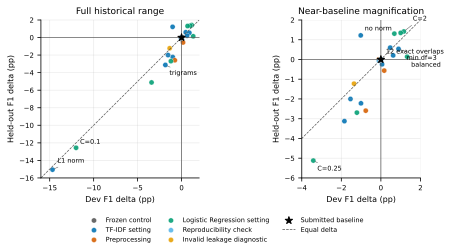
\includegraphics[width=0.94\textwidth]{figure_06_ticket1_dev_probe_deltas.png}
\caption{Ticket 1 historical probe deltas. Each point is the target-1 F1 difference from the submitted baseline, in percentage points, with dev on the horizontal axis and held-out on the vertical axis. The left panel preserves extreme failures; the right panel magnifies near-baseline behavior. The 12 exact overlaps at $(0,0)$ are distinct baseline-equivalent configurations. These post-mismatch held-out records are descriptive diagnostics, not selection evidence.}
\label{fig:ticket1-probe-deltas}
\end{figure*}

The row-level probes show boundary sensitivity without supplying a causal explanation. Dev ID 5282 changed from a correct positive at 0.500826 under the baseline to a false negative at 0.498597 under \texttt{liblinear}. The movement is consistent with a solver-dependent boundary change, but one row does not establish which configuration produced the undisclosed reference.

\subsection{Ticket 2: Text Normalization}

\textbf{Hypotheses and lever.} Ticket 2 asked whether canonicalizing URLs, mentions, hashtags, punctuation, case, or emoji would remove nuisance variation without erasing useful evidence. Each scored candidate enabled exactly one transformation; the raw control reproduced Ticket 1. The intended decision required both dev evidence and a perturbation mechanism, rather than a score alone.

\begin{table*}[t]
\centering
\caption{Ticket 2 Normalization and Invariance Results on Dev}
\label{tab:normalization}
\begin{adjustbox}{max width=\textwidth}
\scriptsize
\begin{tabular}{lrrrrrrrr}
\hline
variant & f1 target 1 & fixed fp & fixed fn & new fp & new fn & robustness affected rows & robustness changed predictions & robustness invariance rate \\
\hline
raw\_text\_control & 0.738812 & 0 & 0 & 0 & 0 & -- & -- & -- \\
normalize\_urls\_placeholder & 0.740313 & 22 & 6 & 11 & 11 & 767 & 0 & 1 \\
normalize\_mentions\_placeholder & 0.736756 & 2 & 1 & 2 & 3 & 399 & 0 & 1 \\
strip\_hashtag\_marker & 0.738812 & 0 & 0 & 0 & 0 & 330 & 0 & 1 \\
normalize\_punctuation\_to\_space & 0.739414 & 1 & 2 & 0 & 2 & 1445 & 0 & 1 \\
unicode\_casefold & 0.738812 & 0 & 0 & 0 & 0 & 1523 & 0 & 1 \\
normalize\_emoji\_placeholder & 0.738812 & 0 & 0 & 0 & 0 & 0 & 0 & 1 \\
\hline
\end{tabular}
\end{adjustbox}
\par\footnotesize{All variants use the frozen baseline model family; robustness values refer to each transformation's matched perturbation. Emoji affected zero dataset rows.}
\end{table*}


\textbf{Dev evidence and decision.} Table~\ref{tab:normalization} shows that URL placeholdering produced the largest normalization F1, 0.740313 versus 0.738812 for raw text. Precision increased from 0.790941 to 0.804659 and accuracy from 0.789232 to 0.793171, while recall decreased from 0.693130 to 0.685496. Relative to Ticket 1 it fixed 22 FPs and 6 FNs, while introducing 11 FPs and 11 FNs. More importantly, on all 767 dev rows subjected to the paired URL substitution, the URL-normalized model changed zero predictions whereas the raw control changed 275. This alignment between the intended lever and measured invariance supported adoption.

Mention placeholdering reduced F1 to 0.736756. Punctuation-to-space gained only 0.000602. Hashtag-marker removal, casefolding, and emoji placeholdering caused no label or metric change. The emoji detector matched zero dataset rows, so this is absence of coverage, not evidence that emoji are useless.

\textbf{Held-out evidence.} After freezing, URL placeholdering achieved precision 0.825137, recall 0.692661, F1 0.753117, and accuracy 0.804990 (Table~\ref{tab:heldout_metrics}). It fixed 22 FPs and 8 FNs but introduced 4 FPs and 15 FNs (Table~\ref{tab:prediction_transitions}). Thus the held-out result preserved the dev mechanism: fewer false positives and higher precision, with a recall cost. The gain remains small, comes from one split, and does not measure the deployment frequency or value of link destinations.

\subsection{Ticket 3: Shortcut and Shallow-Feature Audit}

\textbf{Hypotheses and lever.} Ticket 3 isolated keyword, location, length, missingness, and surface-count blocks, then combined declared subsets with text. The hypothesis was that metadata might contain real benchmark signal while also encoding collection artifacts unlikely to remain stable outside the benchmark. A predeclared trust rule allowed rejection of the highest dev score if targeted perturbations exposed strong shortcut dependence.

\begin{table*}[t]
\centering
\caption{Ticket 3 Shortcut and Shallow-Feature Audit on Dev}
\label{tab:shortcut_audit}
\begin{adjustbox}{max width=\textwidth}
\scriptsize
\begin{tabular}{lrrrrrr}
\hline
variant & f1 target 1 & prediction changes & keyword mask changed predictions & keyword mask f1 & neutralized changed predictions & neutralized f1 \\
\hline
train\_majority\_floor & 0 & 574 & -- & -- & -- & -- \\
raw\_text\_tfidf\_logistic\_regression & 0.738812 & 0 & -- & -- & 99 & 0.721053 \\
keyword\_only & 0.659859 & 378 & 905 & 0.601469 & -- & -- \\
length\_only & 0.437613 & 515 & -- & -- & 297 & 0.249110 \\
keyword\_plus\_length & 0.665060 & 338 & 929 & 0.601656 & 125 & 0.620567 \\
location\_only & 0.224414 & 548 & -- & -- & -- & -- \\
keyword\_plus\_location & 0.658635 & 380 & 902 & 0.603263 & -- & -- \\
selected\_shallow\_only & 0.530290 & 442 & 1003 & 0.605042 & 242 & 0.520158 \\
text\_plus\_keyword & 0.735084 & 148 & 468 & 0.680352 & 77 & 0.714044 \\
text\_plus\_selected\_shallow\_features & 0.749396 & 164 & 702 & 0.642306 & 82 & 0.733068 \\
\hline
\end{tabular}
\end{adjustbox}
\par\footnotesize{Candidate metrics and matched perturbation outcomes are kept on dev. Blank robustness cells mean the perturbation was not applicable to that variant.}
\end{table*}


\textbf{Dev evidence and decision.} Keyword-only F1 was 0.659859, length-only 0.437613, location-only 0.224414, and selected-shallow-only 0.530290 (Table~\ref{tab:shortcut_audit}). Text plus keyword scored 0.735084, below text-only. Text plus keyword and selected shallow features reached the largest visible value, 0.749396, fixing 41 FPs and 46 FNs while introducing 42 FPs and 35 FNs over 164 changed predictions.

That aggregate gain failed the robustness criterion. Masking keyword changed 702 predictions and reduced the rich candidate's F1 to 0.642306. Neutralizing superficial text changed 82 predictions and reduced F1 to 0.733068. For comparison, the text-only model under the same superficial neutralization scored 0.721053. The results show association with keyword availability, not a causal decomposition of feature importance; mask-to-missing is also a severe stress test. Nevertheless, the dependence was strong enough to reject the rich candidate and retain the Ticket 1 text-only model. Ticket 3 therefore reused Ticket 1 held-out predictions without refitting.

The stable-ID cases expose the shortcut mechanism. Keyword-only assigned the same 0.663488 score to dev ID 7, a positive wildfire report whose missing-keyword representation corrected a baseline FN, and ID 25, the negative text ``Summer is lovely,'' where the same representation created an FP. Rich-model ID 331, a figurative concert description containing ``annihilated,'' moved from a correct negative score 0.418088 to an FP at 0.521747. These examples do not estimate prevalence, but they explain why the higher score was not accepted automatically.

\subsection{Ticket 4: Decision Rule and Model}

\textbf{Hypotheses and lever.} Ticket 4 held the raw-text TF--IDF representation fixed while evaluating 61 thresholds from 0.20 through 0.80, seven unweighted Logistic Regression values $C\in\{0.25,0.5,1,2,4,5,10\}$, balanced Logistic Regression at $C\in\{1,5,10\}$, and one LinearSVC comparator at $C=1$. The threshold candidate uses the unweighted $C=1$ scores; all other candidates use their native default rule. Lower thresholds and balanced weighting were expected to raise recall at a precision cost, while regularization and LinearSVC could change sparse-feature separation.

\begin{table*}[t]
\centering
\caption{Ticket 4 Model and Decision-Rule Comparison on Dev}
\label{tab:model_comparison}
\begin{adjustbox}{max width=\textwidth}
\scriptsize
\begin{tabular}{lrrrrrrrrr}
\hline
variant & classifier family & class weight & decision threshold & precision target 1 & recall target 1 & f1 target 1 & accuracy & fixed fn & new fp \\
\hline
lr\_c1\_unweighted\_default & logistic\_regression & -- & 0.500000 & 0.790941 & 0.693130 & 0.738812 & 0.789232 & 0 & 0 \\
lr\_c025\_unweighted\_default & logistic\_regression & -- & 0.500000 & 0.811133 & 0.622901 & 0.704663 & 0.775443 & 5 & 6 \\
lr\_c05\_unweighted\_default & logistic\_regression & -- & 0.500000 & 0.791367 & 0.671756 & 0.726672 & 0.782666 & 3 & 4 \\
lr\_c2\_unweighted\_default & logistic\_regression & -- & 0.500000 & 0.793867 & 0.711450 & 0.750403 & 0.796454 & 16 & 9 \\
lr\_c4\_unweighted\_default & logistic\_regression & -- & 0.500000 & 0.786555 & 0.714504 & 0.748800 & 0.793828 & 22 & 22 \\
lr\_c5\_unweighted\_default & logistic\_regression & -- & 0.500000 & 0.782392 & 0.719084 & 0.749403 & 0.793171 & 25 & 25 \\
lr\_c10\_unweighted\_default & logistic\_regression & -- & 0.500000 & 0.777778 & 0.716031 & 0.745628 & 0.789888 & 28 & 34 \\
lr\_c1\_balanced\_default & logistic\_regression & balanced & 0.500000 & 0.746988 & 0.757252 & 0.752085 & 0.785292 & 42 & 48 \\
lr\_c5\_balanced\_default & logistic\_regression & balanced & 0.500000 & 0.751543 & 0.743511 & 0.747506 & 0.783979 & 37 & 47 \\
lr\_c10\_balanced\_default & logistic\_regression & balanced & 0.500000 & 0.753846 & 0.748092 & 0.750958 & 0.786605 & 41 & 51 \\
linear\_svc\_c1\_default & linear\_svc & -- & 0 & 0.772803 & 0.711450 & 0.740859 & 0.785949 & 27 & 43 \\
lr\_c1\_unweighted\_tuned\_threshold & logistic\_regression & -- & 0.470000 & 0.777049 & 0.723664 & 0.749407 & 0.791858 & 20 & 16 \\
\hline
\end{tabular}
\end{adjustbox}
\par\footnotesize{All rows preserve the frozen text representation; only the listed classifier/regularization/class-weight/threshold lever changes.}
\end{table*}


\begin{figure*}[t]
\centering
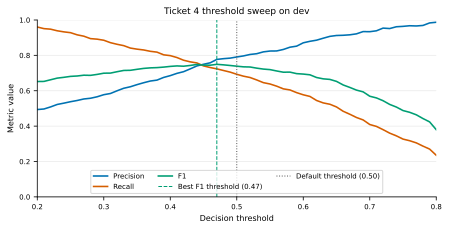
\includegraphics[width=0.94\textwidth]{figure_01_threshold_sweep.png}
\caption{Ticket 4 dev threshold sweep for the unweighted baseline scores. Precision increases and recall decreases as the threshold rises; F1 peaks at 0.47. The balanced model was evaluated separately and selected at the default threshold 0.50. The plotted source contains all 61 verified thresholds.}
\label{fig:threshold}
\end{figure*}

\begin{figure*}[t]
\centering
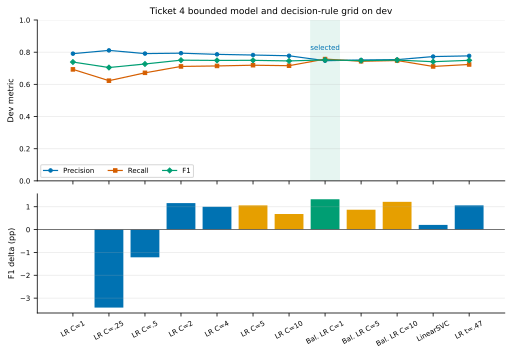
\includegraphics[width=0.94\textwidth]{figure_05_ticket4_model_grid.png}
\caption{Ticket 4 dev model grid. The upper panel preserves the full $[0,1]$ metric scale; the lower panel exposes F1 changes in percentage points relative to unweighted $C=1$. Green marks the frozen selection and orange marks the $C=5/10$ extensions. The extensions are reported as sensitivity evidence because the plan records a historical V1 held-out observation as their motivation.}
\label{fig:model-grid}
\end{figure*}

\textbf{Dev evidence and decision.} Figure~\ref{fig:threshold} shows the expected precision--recall exchange across the baseline threshold sweep. The best threshold-only candidate was 0.47 with F1 0.749407. Figure~\ref{fig:model-grid} and Table~\ref{tab:model_comparison} show that regularization was not monotonic: unweighted $C=2$ reached F1 0.750403 and the highest accuracy, 0.796454, while unweighted $C=5$ and $C=10$ reached 0.749403 and 0.745628. The balanced $C=10$ extension reached F1 0.750958 with precision 0.753846 and recall 0.748092, but did not exceed balanced $C=1$. LinearSVC achieved F1 0.740859.

The pre-execution plan records that the four $C=5/10$ rows were historically motivated by a parallel V1 held-out observation. They are therefore reported as exploratory sensitivity evidence, not as an independent confirmation of the selection rule. Crucially, their inclusion did not determine the final choice: balanced $C=1$ remains the dev-F1 maximum both in the original eight-candidate core and across the full recorded 12-candidate grid. It achieved F1 0.752085, precision 0.746988, and recall 0.757252, fixed 42 baseline FNs, and introduced 48 FPs. It was frozen at $C=1$, balanced weights, and inclusive threshold 0.50.

\textbf{Held-out evidence.} The balanced model achieved precision 0.744361, recall 0.756881, F1 0.750569, and accuracy 0.783979. Relative to Ticket 1, F1 increased only 0.001383, precision fell 0.057033, recall rose 0.053517, and accuracy fell 0.013789. It fixed 35 FNs and introduced 56 FPs, with no fixed FPs or new FNs. This is a defensible F1-oriented, recall-heavy operating point under the declared rule, not an unequivocally superior classifier. No deployment cost function determines whether 35 recovered positives outweigh 56 new false alarms.

\subsection{Ticket 5: Data Quality and Error Audit}

\textbf{Hypotheses and lever.} Ticket 5 asked whether duplicate relationships, likely mislabels, ambiguity, hard negatives, or model weaknesses limited score interpretation, and whether a bounded correction intervention should alter the frozen model. Raw-exact conflicts were treated as evidence of annotation inconsistency. URL-canonical and bounded character-ngram near relationships were candidate generators requiring review. Model disagreement alone was never treated as proof of a wrong label. The only model lever was a single eight-row, train-only label proposal set tested in memory; dev and held-out labels remained untouched.

\begin{table*}[t]
\centering
\caption{Ticket 5 Data-Quality Audit Summary}
\label{tab:data_quality}
\begin{adjustbox}{max width=\textwidth}
\scriptsize
\begin{tabular}{lrrrrr}
\hline
scope & relationship type & groups or pairs & member rows & conflicting groups or pairs & cross split groups or pairs \\
\hline
train\_plus\_dev & exact & 50 & 124 & 13 & 19 \\
train\_plus\_dev & canonical & 214 & 677 & 46 & 98 \\
train\_plus\_dev & near & 693 & 538 & 104 & 265 \\
full\_with\_heldout & exact & 69 & 179 & 18 & 41 \\
full\_with\_heldout & canonical & 292 & 932 & 64 & 194 \\
full\_with\_heldout & near & 960 & 715 & 186 & 546 \\
audit\_disposition & ambiguous & -- & 15 & -- & -- \\
audit\_disposition & fix & -- & 30 & -- & -- \\
audit\_disposition & keep\_but\_flag & -- & 6 & -- & -- \\
audit\_disposition & reject\_false\_positive & -- & 13 & -- & -- \\
\hline
\end{tabular}
\end{adjustbox}
\par\footnotesize{Duplicate rows report groups/pairs and member tweets; disposition rows report audited tweet counts. Source and held-out labels remain unchanged.}
\end{table*}


\textbf{Dev evidence and decision.} On train plus dev, the audit found 50 exact groups with 124 members, 13 conflicting groups, and 19 cross-split groups; 214 canonical groups with 677 members, 46 conflicts, and 98 cross-split groups; and 693 near pairs covering 538 unique IDs, with 104 conflicting and 265 cross-split pairs (Table~\ref{tab:data_quality}). The eight-row correction candidate achieved precision 0.742129, recall 0.755725, F1 0.748865, accuracy 0.782009, and $696/172/160/495$ confusion counts. It reduced F1 by 0.003220, failing the predeclared $-0.002$ noninferiority margin. It fixed 3 errors and introduced 8---7 FPs and 1 FN---so it also failed the error-balance gate. The decision was to retain Ticket 4 with an empty correction list.

\textbf{Post-freeze audit evidence.} After freeze, full-data discovery found 69 exact groups/179 members, 292 canonical groups/932 members, and 960 near pairs covering 715 unique IDs. Cross-split counts were 41, 194, and 546 respectively. These categories overlap and near pairs are candidates, so counts must not be added as unique leakage totals. The final 64-row audit contains 30 \texttt{fix}, 15 \texttt{ambiguous}, 6 \texttt{keep\_but\_flag}, and 13 \texttt{reject\_false\_positive} dispositions. ``Fix'' means a recommendation only. The audit manifest confirms that no source or held-out label was changed and no held-out row was removed.

\subsection{Frozen Final Choice and Cross-Ticket Interpretation}

Figure~\ref{fig:dev-heldout} compares dev and held-out F1 without changing the decision rule. Tickets 1 and 3 share one prediction core; Tickets 4 and 5 share the final core. Ticket 2 has the largest observed held-out F1, but using that observation to replace Ticket 5 would be held-out tuning. The valid final identity is therefore Ticket 5: the Ticket 4 balanced Logistic Regression recipe with no training-label corrections.

\begin{figure*}[t]
\centering
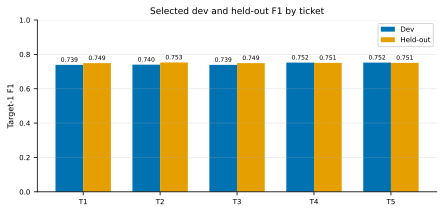
\includegraphics[width=0.94\textwidth]{figure_02_dev_heldout_f1.png}
\caption{Selected dev and post-freeze held-out target-1 F1 by ticket. The full $[0,1]$ axis avoids exaggerating small differences. T1/T3 and T4/T5 are intentional shared prediction cores; held-out bars are descriptive rather than a new selection criterion.}
\label{fig:dev-heldout}
\end{figure*}

Figure~\ref{fig:transitions} makes the semantic cost clearer than F1 alone. URL placeholdering mainly removes FPs but also creates FNs. Balanced weighting recovers FNs at the cost of more new FPs. A single net error count would conceal this directional difference.

\begin{figure*}[t]
\centering
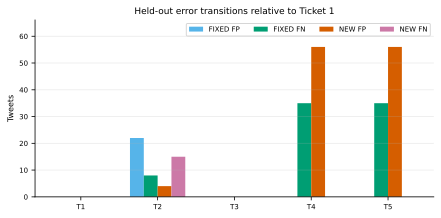
\includegraphics[width=0.94\textwidth]{figure_03_prediction_transitions.png}
\caption{Held-out fixed and newly introduced error counts relative to Ticket 1. Counts begin at zero and remain separated by error type.}
\label{fig:transitions}
\end{figure*}

\section{Case Analysis}

\subsection{Prediction Movements that Match Intended Levers}

Table~\ref{tab:cases} deliberately contains favorable and unfavorable cases. For URL placeholdering, held-out ID 773 is a target-0 advertising tweet with two links. Its baseline FP score 0.533045 falls to 0.460680, fixing the error. Conversely, ID 902 is a target-1 bioterrorism report whose score falls from 0.508666 to 0.499356, creating an FN. The pair is consistent with a transformation that removes link-string sensitivity but can move borderline positives below threshold.

For balanced weighting, held-out ID 556 is a target-1 arson-related example whose score rises from 0.464323 to 0.529717, fixing an FN. ID 59 is a target-0 link-heavy post whose score rises from 0.450541 to 0.504457, creating an FP. These cases instantiate the recall--precision exchange in Table~\ref{tab:prediction_transitions}. ID 767 is another verified new FP. Its machine-generated scores are 0.487623 and 0.544815; older narrative values conflict with the transition CSV and are not used.

The Ticket 5 correction probe is similarly mixed. Dev ID 9470 moves from an FP at 0.633044 to a correct negative at 0.465278, but ID 4014 moves from a correct negative at 0.496509 to an FP at 0.502209. The aggregate gate correctly prevented a small set of plausible semantic edits from being presented as an unqualified model improvement.

\begin{table*}[t]
\centering
\caption{Representative Successes, Failures, Ambiguities, and Audit Cases}
\label{tab:cases}
\begin{adjustbox}{max width=\textwidth}
\scriptsize
\begin{tabular}{lrrrrrrrrr}
\hline
ticket & split & id & case type & true label & baseline pred & baseline score & candidate pred & candidate score & transition or disposition \\
\hline
1 & dev & 5282 & solver boundary failure & 1 & 1 & 0.500826 & 0 & 0.498597 & new\_error \\
2 & heldout & 773 & normalization success & 0 & 1 & 0.533045 & 0 & 0.460680 & fixed\_error \\
2 & heldout & 902 & normalization failure & 1 & 1 & 0.508666 & 0 & 0.499356 & new\_error \\
3 & dev & 7 & shortcut success & 1 & 0 & 0.412138 & 1 & 0.663488 & fixed\_error \\
3 & dev & 25 & shortcut failure & 0 & 0 & 0.265330 & 1 & 0.663488 & new\_error \\
3 & dev & 331 & shallow-feature failure & 0 & 0 & 0.418088 & 1 & 0.521747 & new\_error \\
4 & heldout & 556 & recall success & 1 & 0 & 0.464323 & 1 & 0.529717 & fixed\_error \\
4 & heldout & 59 & precision failure & 0 & 0 & 0.450541 & 1 & 0.504457 & new\_error \\
4 & heldout & 767 & verified score conflict & 0 & 0 & 0.487623 & 1 & 0.544815 & new\_error \\
5 & dev & 9470 & correction-probe success & 0 & 1 & 0.633044 & 0 & 0.465278 & fixed\_error \\
5 & dev & 4014 & correction-probe failure & 0 & 0 & 0.496509 & 1 & 0.502209 & new\_error \\
5 & heldout & 5760 & validated model error & 0 & -- & -- & 1 & 0.768287 & reject\_false\_positive \\
5 & heldout & 2619 & potential annotation issue & 1 & -- & -- & 0 & 0.224300 & fix \\
5 & heldout & 6220 & ambiguity & 0 & -- & -- & 1 & 0.645703 & ambiguous \\
5 & heldout & 6223 & ambiguity & 1 & -- & -- & 1 & 0.645703 & ambiguous \\
5 & heldout & 10795 & validated model error & 1 & -- & -- & 0 & 0.135000 & reject\_false\_positive \\
\hline
\end{tabular}
\end{adjustbox}
\par\footnotesize{The CSV preserves full text, scores, and rationales; the compact report table preserves the verified numeric case ledger. Stable IDs support exact lookup.}
\end{table*}


\subsection{Hard Negatives, Potential Annotation Issues, and Ambiguity}

Error direction does not adjudicate a label. Held-out ID 5760 explicitly says there are ``no forest fires.'' The final model predicts positive at 0.768287, but the audit rejects the suspicion that the negative label is wrong; this is a valid hard negative and a model error involving negation. ID 10795, a target-1 report about a wrecked home, is predicted negative at 0.135000; the audit likewise treats it as model weakness rather than a mislabel.

By contrast, held-out ID 2619 is labeled target 1 but says ``My iPod crashed'' with fan hashtags. The audit recommends a potential 1-to-0 fix, but no external adjudicator confirmed it and the source label remains unchanged. IDs 6220 and 6223 contain identical text about the historical D. B. Cooper image but have opposite held-out labels. Since the evidence is identical, both are marked ambiguous and unsuitable for automatic correction. These cases show why the four-way audit vocabulary separates recommendation, ambiguity, flagging, and rejection.

\begin{figure}[t]
\centering
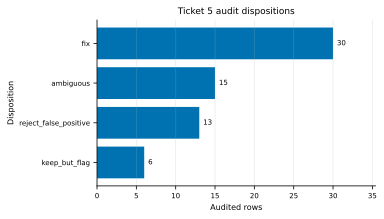
\includegraphics[width=\columnwidth]{figure_04_data_quality_dispositions.png}
\caption{Disposition counts in the 64-row data-quality audit. ``Fix'' denotes a recommendation, not an applied label mutation.}
\label{fig:data-quality}
\end{figure}

Figure~\ref{fig:data-quality} summarizes the curated audit, not the prevalence of defects in all 7,613 rows. Its 64 records were selected for review and the near-duplicate search was bounded. The semantic judgments are human/AI-supported assessments without independent expert or multi-annotator ground truth.

\subsection{Why Aggregate Improvement Is Insufficient}

The case and robustness evidence support a consistent conclusion. Ticket 2's small gain accompanies both fixed and new errors. Ticket 3's largest visible dev score depends strongly on keyword availability. Ticket 4's F1 choice recovers positives while adding more false alarms and lowering accuracy. Ticket 5 shows that apparently plausible corrections can reduce agreement with the benchmark. Thus a higher F1 can coexist with shortcut fragility, undesirable operating costs, or contradictory labels. Trustworthiness in this report means convergence among controlled dev selection, expected directional movements, targeted robustness, stable-ID examples, and freeze provenance. It is not a formal statistical proof or deployment guarantee.

\section{Difficulties and Solutions}

Table~\ref{tab:difficulties} records six difficulties supported by machine artifacts. Three were especially consequential.

First, the literal baseline missed the reference but the reference exposed too little evidence to isolate a cause. The response was to verify ID alignment, train-only fitting, convergence, effective settings, seeds, versions, and 32 one-lever probes, then preserve the mismatch as unresolved rather than invent a causal explanation. The later Ticket 1 artifact reconstruction was qualified as one exact frozen-recipe recovery replay, not another selection round. The complete prior deletion history cannot be independently reconstructed because usable Git history is absent.

Second, the largest Ticket 3 dev gain appeared attractive until targeted masking exposed dependency on keyword availability. Adding robustness probes converted a score comparison into an evidence-based rejection. This solution remains bounded: the probes cover predefined feature families and severe perturbations, not every possible shortcut.

Third, Ticket 4 required selecting an operating point without held-out tuning. The solution was a predeclared dev criterion, a complete 61-threshold curve, bounded classifier candidates, confusion matrices, and fixed/new error analysis before freezing. The resulting choice is described as recall-oriented because the artifacts show both its benefit and cost.

Data quality created a fourth difficulty: duplicate conflicts, ambiguity, and model weakness cannot be separated by prediction error alone. Exact/canonical/near discovery was therefore separated from four allowed dispositions, and label proposals were tested only in memory under a dev gate. Finally, replay produced maximum probability drift of $1.11\times10^{-16}$ despite identical labels and metrics. Verification used a $10^{-12}$ score tolerance, exact stable-ID/label/order checks, and a $10^{-15}$ metric tolerance rather than falsely requiring cross-library byte identity.

\begin{table*}[t]
\centering
\caption{Verified Project Difficulties, Responses, and Residual Limits}
\label{tab:difficulties}
\scriptsize
\setlength{\tabcolsep}{3pt}
\renewcommand{\arraystretch}{1.08}
\begin{tabular}{@{}p{0.18\textwidth}p{0.22\textwidth}p{0.31\textwidth}p{0.22\textwidth}@{}}
\hline
\textbf{difficulty} & \textbf{verified evidence} & \textbf{response} & \textbf{residual limit} \\
\hline
Assignment reference and frozen baseline did not match & Held-out absolute F1 gap=0.00823649010418; tolerance=0.001. & Ran isolated dev probes and structural checks, then retained the reproducible frozen implementation and documented the unresolved gap. & The assignment's hidden reference pipeline remains unknown. \\
Score-level numerical drift under clean replay & Final replay audit records stable labels/order and bounded score drift. & Compared hashes, stable IDs, labels, metrics, and score differences under explicit tolerances. & Exact floating-point identity is not claimed. \\
Apparent dev gain depended on shortcut-prone features & Matched keyword masking and superficial-text neutralization materially changed predictions and F1. & Rejected the richer candidate and retained the text-only frozen baseline. & The audit covers predefined shallow features and perturbations, not every possible shortcut. \\
Recall gains created precision costs & Balanced Logistic Regression fixes false negatives while introducing false positives on dev and held-out. & Evaluated bounded candidates, a full threshold sweep, confusion matrices, and transition counts before freezing the default-threshold balanced model. & The operating point reflects target-1 F1, not a deployment cost function. \\
Duplicate conflicts and ambiguous annotations & Duplicate summaries and 64 stable-ID audit records include conflicts and four dispositions. & Kept source/held-out labels unchanged, separated fix/ambiguous/keep/reject dispositions, and gated a train-only correction probe on dev. & Audit dispositions are evidence assessments, not ground-truth adjudications. \\
Emoji normalization lacked dataset coverage & The matched robustness artifact reports zero affected dev rows. & Retained the zero-coverage result and did not infer a dataset-level benefit. & The emoji hypothesis remains unresolved on this split. \\
\hline
\end{tabular}
\par\footnotesize{Only difficulties supported by generated artifacts are included; narrative-only events are excluded.}
\end{table*}


\section{AI Usage Declaration}

OpenAI Codex was used as the repository-operating AI assistant \cite{openai-codex}. No retained evidence establishes the use of an independent labeling agent or external expert service. Codex assisted with repository inspection, requirement decomposition, implementation planning, Python and test drafting, controlled experiment orchestration after user authorization, artifact review, reproducibility auditing, and report preparation. The retained interaction record is a curated reconstruction supported by files and commands; it is not a verbatim export of all messages or hidden model reasoning.

AI-generated material was not accepted automatically. Code and experiment suggestions were accepted only when executable tests and artifact checks passed. Interpretations were changed or rejected when row-level evidence disagreed: for example, the stale narrative scores for ID 767 were rejected in favor of the machine transition CSV, unsupported explanations for the Ticket 1 reference gap were omitted, and semantic Ticket 5 ``fix'' judgments remained recommendations rather than source edits. Higher-scoring empirical candidates were also rejected when the predeclared evidence rules failed, as in Ticket 3's shortcut-sensitive rich model and Ticket 5's correction probe.

Verification included schema and stable-ID tests; train/dev/held-out separation checks; deterministic hashes; prediction-level recomputation of precision, recall, F1, accuracy, confusion counts, and transitions; freeze chronology; source-label integrity; and five clean-process replays. The retained validation record reports 56 passing tests, no broken package requirements, a non-refitting submission-validator PASS, five reproduced ticket cores, and byte-exact regeneration of the three active result tables. The report-asset generator added 206 assertions over source hashes, archived prediction hashes, schemas, row counts, stable IDs, labels, configurations, metrics, cases, and source paths.

Human responsibility remains explicit. The user authorized major stages and held-out/audit actions. AI suggestions did not provide independent ground truth. The submitter must verify the final author metadata, citations, wording, and course-policy compliance, and must review semantic audit judgments before submission. Table~\ref{tab:ai_usage} summarizes this division of labor.

\begin{table*}[t]
\centering
\caption{AI Usage and Verification Workflow}
\label{tab:ai_usage}
\scriptsize
\setlength{\tabcolsep}{3pt}
\renewcommand{\arraystretch}{1.08}
\begin{tabular}{@{}p{0.16\textwidth}p{0.25\textwidth}p{0.34\textwidth}p{0.18\textwidth}@{}}
\hline
\textbf{workflow stage} & \textbf{ai assistance} & \textbf{verification} & \textbf{human accountability} \\
\hline
Evidence and contract audit & Repository inspection, requirement decomposition, and artifact inventory & Claims cross-checked against handout, clarifications, generated CSV/JSON, predictions, and frozen manifests & Final interpretation and submission remain the student's responsibility \\
Implementation and testing & Pipeline/test drafting and diagnostic support & Automated tests, deterministic split checks, artifact schemas, hashes, and row-level assertions & No AI statement is accepted when it conflicts with machine-generated artifacts \\
Experiment orchestration & Running authorized dev experiments and producing frozen artifacts & Selections use dev evidence; held-out completion files and frozen manifests enforce usage policy & Held-out results did not reopen ticket selection \\
Reproducibility audit & Clean-process replay and comparison of archived outputs & Five tickets reproduced with stable IDs, labels, metrics, transitions, and bounded score tolerances & Exact score identity is not overstated \\
Report asset generation & Programmatic table, figure, and case-material generation & This script recomputes metrics, verifies labels/IDs/configuration, and records an asset manifest & Generated assets must be reviewed before inclusion \\
\hline
\end{tabular}
\par\footnotesize{This is a workflow declaration, not a substitute for source citations or human review.}
\end{table*}


\section{Discussion and Limitations}

\subsection{What Evidence Is Trustworthy}

The strongest evidence in this project combines several independent constraints. Ticket 2 was adopted because a small dev gain aligned with a directly measured URL-invariance mechanism and a precision-oriented transition pattern that persisted after freeze. Ticket 3 was rejected because its higher score conflicted with robustness evidence. Ticket 4 was adopted cautiously because it won the declared dev criterion and its predicted recall mechanism persisted, although its held-out F1 advantage was small. Ticket 5 rejected corrections because both the noninferiority and error-balance gates failed. These different decisions demonstrate that ``highest score'' and ``most trustworthy evidence'' are not synonyms.

Internal reproducibility is strong within the locked environment. Five isolated processes reproduced all selected labels; maximum score drift was $1.11\times10^{-16}$, below the $10^{-12}$ tolerance. The summary, threshold sweep, and data-quality audit regenerated byte-for-byte. Final predictions contain 1,523 unique held-out IDs in the fixed order. This supports the provenance of the reported observations, but it does not validate the benchmark labels or prove cross-platform bit identity.

\subsection{Remaining Uncertainty and Risks}

The Ticket 1 discrepancy remains causally unresolved because the supplied reference is a scalar without prediction-level or configuration evidence. Small differences among candidates are based on one dev split; the project contains no bootstrap, repeated split, confidence interval, or formal significance analysis. Text duplicates and approximate relationships violate an independence intuition even though stable IDs are disjoint. No duplicate-group-aware evaluation estimates how performance changes when related text is kept within one partition.

Ticket 3 perturbations are severe and benchmark-specific. Keyword coefficients and score movements are associations rather than causal importance measures. Ticket 4 explores a finite grid and one alternative classifier; it has no calibrated deployment cost for false alarms versus misses. Ticket 5's canonicalization can hide URL-destination information, and its near-duplicate search uses at most seven non-self neighbors at one threshold and representation. The 64 semantic audit records are curated rather than exhaustive, and no expert multi-annotator adjudication exists. Links were not fetched, so destination context was not verified.

The hidden-test risk follows directly from these limits. Superficial URL, keyword, location, missingness, and length patterns can be perturbed without changing intended labels. The accepted URL transformation has a measured invariance benefit, whereas the rejected rich model shows substantial keyword sensitivity. Nevertheless, neither experiment proves robustness to all hidden variants, temporal drift, new disasters, changing platform conventions, or different label policies.

\subsection{Final Model Interpretation and External Validity}

The final model is the last valid dev-based frozen choice: raw word-unigram TF--IDF plus balanced Logistic Regression at $C=1$ and threshold 0.50, with no label corrections. It is recall-oriented. Relative to Ticket 1 on held-out, recall increases from 0.703364 to 0.756881 while precision decreases from 0.801394 to 0.744361 and accuracy from 0.797768 to 0.783979. The F1 gain is only 0.001383. These observations justify the procedural choice under the declared F1 criterion, not a universal operational optimum.

A deployment decision would require explicit costs, external or temporal validation, duplicate-aware splitting, threshold calibration under the deployment base rate, and a clearer annotation policy. Ticket 2's higher observed held-out F1 is a useful result, but choosing it post hoc would compromise the study's held-out discipline. The report therefore preserves the final frozen identity rather than rewriting the conclusion around the most favorable visible score.

\section{Conclusion}

This forensic study found that the local raw-text TF--IDF plus Logistic Regression baseline is reproducible and leakage-controlled but does not match the undisclosed reference within tolerance. URL placeholdering is a defensible isolated surface lever because a small precision-oriented gain aligns with exact paired perturbation invariance. Shallow-feature augmentation is not adopted despite a higher dev F1 because the gain is strongly keyword-sensitive. Balanced Logistic Regression changes the operating point toward recall and wins the declared dev F1 criterion, but its held-out advantage is small, precision and accuracy fall, and new FPs exceed recovered FNs. Duplicate conflicts and ambiguous labels materially limit score interpretation, yet the tested eight-label correction set worsens dev evidence and is rejected.

The final frozen decision is therefore balanced Logistic Regression at the default threshold with no label corrections. The central lesson is methodological: aggregate scores become credible only when connected to controlled levers, fixed and newly introduced errors, robustness probes, stable-ID cases, frozen chronology, and reproducible artifacts. Even that evidence remains bounded by one benchmark, one fixed split, unresolved reference details, duplicate dependence, and unadjudicated labels.

\bibliographystyle{IEEEtran}
\bibliography{references}

\appendices

\section{Extended Configurations and Negative Results}

Ticket 1's complete probe artifacts show that lowercasing off, bigrams, \texttt{liblinear}, $C=0.5$, and an intentionally leaky train-plus-dev vocabulary all reduced dev F1. Raising \texttt{max\_iter}, changing the seed, and spelling L2 explicitly produced no label change. These negative and null results constrain explanations but do not reveal the undisclosed reference implementation.

Ticket 2's full normalization table is Table~\ref{tab:normalization}. Mention placeholdering was negative; punctuation-to-space was only marginally positive; hashtag stripping, casefolding, and emoji placeholdering were label-equivalent to raw text. Ticket 3's full ten-row comparison is Table~\ref{tab:shortcut_audit}. The isolated keyword, location, length, and shallow families were all weaker than text-only, while the rich model's visible gain failed robustness. Ticket 4's complete 12-row model table is Table~\ref{tab:model_comparison}; $C=0.25$ and $C=0.5$ hurt, the $C=5/10$ extensions did not surpass balanced $C=1$, LinearSVC did not win, and both threshold 0.47 and unweighted $C=2$ lost to balanced weighting under the declared dev criterion. The extended rows are exploratory because of their documented V1 motivation. These are bounded comparisons on one split, not exhaustive searches.

\section{Data-Quality and Correction Detail}

Raw-exact relationships require identical stored text. Canonical relationships use deterministic text canonicalization, including URL handling, to identify closely related reposts. Near relationships are bounded character-ngram candidates rather than proof of equivalence. Categories overlap. Audit records use four dispositions: \texttt{fix} for a supported recommendation, \texttt{ambiguous} when evidence cannot resolve a label, \texttt{keep\_but\_flag} for a retained row with a documented concern, and \texttt{reject\_false\_positive} when a suspicion of data error is rejected.

The correction probe contained eight stable training IDs: 4076, 6566, 8698, 8739, 1723, 1760, 6097, and 9472. Original and proposed labels were preserved side by side, and only an in-memory training copy changed. The candidate failed its dev gates, so none of the proposals was applied to source data. Rejection of the candidate does not prove that all original labels are semantically correct; it shows only that the bundled intervention was not justified for the frozen classifier under the declared dev criteria.

\section{Stable-ID Case and Evidence Provenance}

\balance

Table~\ref{tab:cases} is the report's extended case ledger. Its CSV source preserves full text, probability values, and selection rationales; the compact report table preserves IDs, labels, predictions, scores, and transition or disposition. Cases were selected from actual transition or audit files and include successes and failures. They are illustrative, not prevalence estimates. Ticket 4 ID 767 uses only the machine-generated scores.

All report tables and figures were generated by \path{scripts/generate_report_assets.py}. The exact source list for each asset is \path{report_assets/asset_manifest.csv}, and the 206 assertion outcomes are in \path{report_assets/validation_report.json}. Central frozen recipes, hashes, archived prediction paths, expected metrics, and transition counts are in \path{configs/frozen_decisions.json}. Run commands remain in per-experiment \texttt{run\_command.txt} files rather than being pasted into this report.

The clean audit recorded five distinct replay processes, identical labels and stable-ID order, maximum score drift $1.11\times10^{-16}$, and no reopened selection. It regenerated \path{results/summary.csv}, \path{results/threshold_sweep.csv}, and \path{results/data_quality_audit.csv} byte-for-byte. The final prediction file is \path{predictions/final-heldout-predictions.csv}. This establishes internal reproducibility under the locked environment; it does not establish bit-identical scores across arbitrary platforms.

\section{Report Finalization Boundaries}

The author names were supplied directly. Unsupplied affiliation, location, and email metadata are omitted rather than inferred. Bibliographic URLs and software versions were checked against official pages where available; course-internal sources use repository filenames because no public metadata was supplied.

\end{document}
